\documentclass[12pt,a4paper]{article}
\usepackage[utf8]{inputenc}
\usepackage{geometry}
\usepackage{graphicx}
\usepackage{amsmath}
\usepackage{hyperref}
\usepackage{titlesec}
\usepackage{changepage}
\usepackage{caption}
\usepackage{float}
\usepackage{booktabs}
\usepackage{tabularx}
\usepackage[numbers]{natbib} % Menambahkan paket natbib untuk referensi
\usepackage{setspace} % Untuk mengatur spasi antar baris

% Page layout
\geometry{top=1in, bottom=1in, left=1in, right=1in}

% Modify section and subsection font size to normal
\titleformat{\section}[hang]{\normalsize\bfseries}{\thesection}{1em}{}
\titleformat{\subsection}[hang]{\normalsize\bfseries}{\thesubsection}{1em}{}

% Hanging indent for references
\setlength{\bibsep}{1em} % Mengatur jarak antar entri referensi
\setlength{\bibhang}{2em} % Mengatur indentasi menggantung untuk referensi

\begin{document}

% Title
\begin{titlepage}
    \centering
    {\Large\textbf{Deep Learning Course \\ Final Project Report}\par} % Judul
    \vspace{2cm} % Jarak antara judul dan logo
    
\includegraphics[width=0.5\linewidth]{Images/Logo_UH.png}\par % Logo
    \vspace{2cm} % Jarak antara logo dan nama
    \textbf{Disusun oleh:}\\[0.5cm]
    {\large
    Rahmatia (H071221004)\\ 
    Muhammad Iswari (H071221007)\\ 
    Vicky Jesflinto (H071221019)\par}
    \vspace{1cm} % Jarak antara nama dan tanggal

    \vfill

    % Informasi universitas dan tanggal
    \textbf{Universitas Hasanuddin}\\
    \textbf{Makassar, Indonesia}\\[0.5cm]
    \textbf{\today}
\end{titlepage}

\normalsize  % Set the text size to normal for the entire document
\tableofcontents
\newpage

% 1. Introduction
\section{INTRODUCTION}

\subsection{Latar Belakang dan Konteks Proyek}
\begin{adjustwidth}{3em}{0pt} 
\hspace{0.5cm} Kerusakan pada bangunan, terutama yang berupa retakan pada permukaan dinding, merupakan salah satu masalah umum yang dapat memengaruhi stabilitas struktural serta keselamatan seseorang dalam suatu bangunan. Retakan pada dinding tidak hanya berpotensi menurunkan nilai estetika pada bangunan, tetapi juga dapat mengindikasikan adanya masalah serius, seperti pergeseran struktural atau kelembapan yang dapat menyebabkan kerusakan lebih lanjut. Jika dibiarkan, sebuah retakan kecil dapat berkembang menjadi retakan yang lebih besar dan dapat menyebabkan masalah. Oleh karena itu, pendeteksian dini terhadap retakan pada permukaan dinding sangat penting untuk mencegah kerusakan yang lebih parah dan mempercepat proses perbaikan.

Seiring perkembangan teknologi, khususnya dalam bidang Deep Learning, deteksi kerusakan pada dinding dapat dilakukan secara otomatis melalui penggunaan model deteksi objek. Pendekatan ini memberikan solusi yang lebih cepat, efisien, dan akurat dalam memantau kondisi dinding, dibandingkan metode tradisional yang mengandalkan inspeksi manual yang membutuhkan banyak waktu.
\end{adjustwidth}

\subsection{Masalah}
\begin{adjustwidth}{3em}{0pt} 
\hspace{0.5cm} Kondisi pada permukaan dinding bangunan, khususnya retakan sering kali tidak terdeteksi dengan cepat, karena terkadang ukurannya yang kecil dan tidak terlihat. Kurangnya dataset tentang kerusakan permukaan dinding terorganisir menjadi salah satu hambatan utama dalam mengembangkan solusi berbasis teknologi. Di sisi lain, deteksi manual terhadap retakan ini memerlukan waktu, tenaga, dan keahlian yang tidak selalu tersedia, serta rentan terhadap kesalahan manusia. Selain itu, proses inspeksi yang lambat dapat menyebabkan keterlambatan dalam penanganan, yang pada akhirnya dapat memperburuk kerusakan dan meningkatkan biaya perbaikan. Tanpa adanya sistem deteksi yang efisien, kerusakan pada dinding dapat berkembang menjadi masalah yang lebih besar, mengancam keselamatan bangunan dan penghuninya.
\end{adjustwidth}

\subsection{Tujuan}
\begin{adjustwidth}{3em}{0pt} 
\hspace{0.5cm} Tujuan dari proyek ini adalah untuk menghasilkan dataset yang menyediakan data yang representatif dalam mendeteksi retakan pada permukaan dinding, seperti dinding mulus, retakan kecil, dan retakan besar menggunakan teknologi deteksi objek. Dengan menggunakan teknik Deep Learning, khususnya model YOLOv5, untuk mendeteksi kerusakan permukaan dinding secara akurat dan efisien. Dengan adanya sistem deteksi otomatis, diharapkan dapat mempercepat proses inspeksi, mengurangi ketergantungan pada inspeksi manual, serta meningkatkan efektivitas dalam mengidentifikasi kerusakan sejak dini, sehingga dapat mencegah kerusakan yang lebih parah dan mengurangi biaya perbaikan.
\end{adjustwidth}

% 2. Related Works
\section{RELATED WORKS}
\begin{adjustwidth}{3em}{0pt} 
\hspace{0.5cm} Deteksi retakan pada permukaan dinding telah menarik perhatian banyak peneliti dalam beberapa tahun terakhir, mengingat pentingnya untuk menjaga integritas struktural bangunan. Berbagai pendekatan, mulai dari metode pengolahan citra konvensional hingga teknik Deep Learning yang lebih modern, telah diusulkan untuk mendeteksi kerusakan tersebut. Berikut adalah tinjauan pustaka mengenai berbagai pendekatan yang relevan dan bagaimana proyek ini membangun atau berbeda dari karya-karya sebelumnya.

\begin{enumerate}
    \item \textbf{Pengolahan Citra Tradisional untuk Deteksi Retakan}
    
    \hspace{0.5cm} Sebelum munculnya Deep Learning, penelitian di bidang deteksi retakan lebih mengandalkan teknik pengolahan citra tradisional. Metode seperti \textbf{edge detection} dan transformasi morfologi telah digunakan untuk menyoroti kontur dan tepi retakan pada permukaan dinding. Misalnya, \textit{Zhang et al. (2016)} menggunakan deteksi tepi berbasis operator Sobel untuk mengidentifikasi retakan pada gambar bangunan. Meskipun metode ini dapat memberikan hasil yang memadai dalam beberapa kondisi, kekurangannya adalah ketidakmampuan untuk menangani keragaman bentuk dan tekstur retakan yang kompleks, serta sensitivitas terhadap pencahayaan dan noise dalam gambar.

    \item \textbf{Pendekatan Machine Learning dengan Fitur Ekstraksi Manual}
    
    \hspace{0.5cm} Beberapa studi menggunakan teknik Machine Learning dengan ekstraksi fitur manual untuk mendeteksi kerusakan pada permukaan dinding. \textit{Saha et al. (2018)}, misalnya, menggunakan algoritma \textbf{Support Vector Machine (SVM)} yang memanfaatkan fitur tekstur dan bentuk retakan. Meskipun hasil yang diperoleh cukup memadai dalam kasus tertentu, pendekatan ini membutuhkan pengolahan fitur secara manual yang sering kali rumit dan membutuhkan waktu. Selain itu, metode ini kurang fleksibel dalam mengatasi kerusakan dengan variasi bentuk, ukuran, dan tekstur yang tinggi.

    \item \textbf{Pendekatan Deep Learning dengan CNN}
    
    \hspace{0.5cm} Seiring dengan kemajuan Deep Learning, beberapa penelitian mulai mengalihkan perhatian ke arsitektur jaringan saraf konvolusional (\textbf{Convolutional Neural Networks - CNN}) untuk deteksi kerusakan pada permukaan dinding. \textit{Li et al. (2020)} mengusulkan penggunaan CNN untuk mendeteksi retakan pada dinding beton dan menunjukkan hasil yang lebih akurat dibandingkan dengan pendekatan sebelumnya. CNN memiliki kemampuan untuk belajar secara otomatis dari data tanpa memerlukan ekstraksi fitur manual, dan telah terbukti unggul dalam mengidentifikasi pola tekstur yang lebih kompleks. \textit{Wang et al. (2021)} juga menggunakan arsitektur \textbf{U-Net}, yang berbasis CNN, untuk segmentasi gambar retakan dan menghasilkan hasil yang sangat akurat, bahkan dalam kondisi pencahayaan yang tidak ideal.

    \hspace{0.5cm} Namun, meskipun CNN memberikan akurasi yang sangat baik dalam klasifikasi citra, ada keterbatasan terkait dengan kecepatan inferensi, terutama dalam aplikasi dunia nyata yang membutuhkan deteksi real-time. Ini mengarah pada pencarian pendekatan yang lebih efisien dalam hal waktu komputasi tanpa mengorbankan akurasi.

    \item \textbf{Penggunaan YOLOv5 dalam Deteksi Objek}
    
    \hspace{0.5cm} Untuk mengatasi keterbatasan deteksi real-time pada arsitektur CNN tradisional, beberapa penelitian mengalihkan fokus ke arsitektur deteksi objek berbasis \textbf{You Only Look Once} (YOLO), terutama versi terbaru yaitu YOLOv5. YOLO adalah model deteksi objek yang dirancang untuk mendeteksi dan mengklasifikasikan objek dalam gambar secara langsung dan dalam satu langkah pemrosesan, yang memungkinkan deteksi cepat dan akurat.

    \hspace{0.5cm} Dalam konteks deteksi retakan pada dinding, YOLOv5 menawarkan beberapa keuntungan dibandingkan CNN tradisional. YOLOv5 lebih cepat dalam melakukan inferensi karena dapat memproses gambar dalam waktu yang lebih singkat, menjadikannya lebih cocok untuk aplikasi real-time. Beberapa studi, seperti yang dilakukan oleh \textit{Redmon et al. (2016)}, menunjukkan bahwa YOLO, khususnya versi terbaru, dapat memberikan akurasi yang sangat baik dalam mendeteksi objek dalam gambar, dengan keunggulan dalam hal kecepatan pemrosesan. Dalam konteks proyek ini, YOLOv5 dipilih karena kemampuannya untuk melakukan deteksi objek secara langsung, yang memungkinkan model untuk mendeteksi dan mengklasifikasikan retakan pada permukaan dinding secara cepat dan efisien, bahkan dalam kondisi gambar yang bervariasi.

    \item \textbf{Pendekatan yang Digunakan dalam Proyek Ini}
    
    \hspace{0.5cm} Proyek ini mengadopsi pendekatan deteksi objek menggunakan YOLOv5 untuk mendeteksi retakan pada permukaan dinding. Meskipun awalnya kami mempertimbangkan penggunaan CNN tradisional, kami memutuskan untuk beralih ke YOLOv5 setelah mempertimbangkan kelebihannya dalam hal kecepatan dan akurasi deteksi objek secara real-time. Dataset \textbf{Wall Surface Crack Texture} yang kami kembangkan berisi gambar-gambar retakan pada dinding dalam berbagai kondisi, yang dirancang untuk melatih model deteksi objek dalam mengenali berbagai bentuk, ukuran, dan tekstur retakan.

    \hspace{0.5cm} Dengan menggunakan YOLOv5, kami tidak hanya memperoleh akurasi yang lebih baik, tetapi juga mengatasi tantangan terkait waktu inferensi yang cepat, yang sangat penting untuk aplikasi praktis dalam inspeksi kondisi bangunan. Pendekatan ini memungkinkan deteksi retakan yang lebih efisien dan lebih cepat dibandingkan dengan metode CNN tradisional yang cenderung lebih lambat dalam pemrosesan gambar secara keseluruhan.
\end{enumerate}
\end{adjustwidth}

% 3. Dataset and Material
\section{DATASET MATERIAL}
\subsection{Dataset}
Dalam proyek ini, kami membuat \textit{dataset} khusus untuk deteksi kerusakan jalan melalui langkah-langkah berikut:

\subsubsection{Sumber Dataset}
\begin{itemize}
    \item Foto Langsung: Gambar kerusakan dinding diambil menggunakan kamera smartphone dari berbagai lokasi untuk menangkap kondisi nyata di lapangan.
    \item Google: Gambar kerusakan jalan diunduh dari pencarian internet, berfokus pada variasi kerusakan jalan dari berbagai negara dan lingkungan.
    \begin{figure}[h]
        \centering
        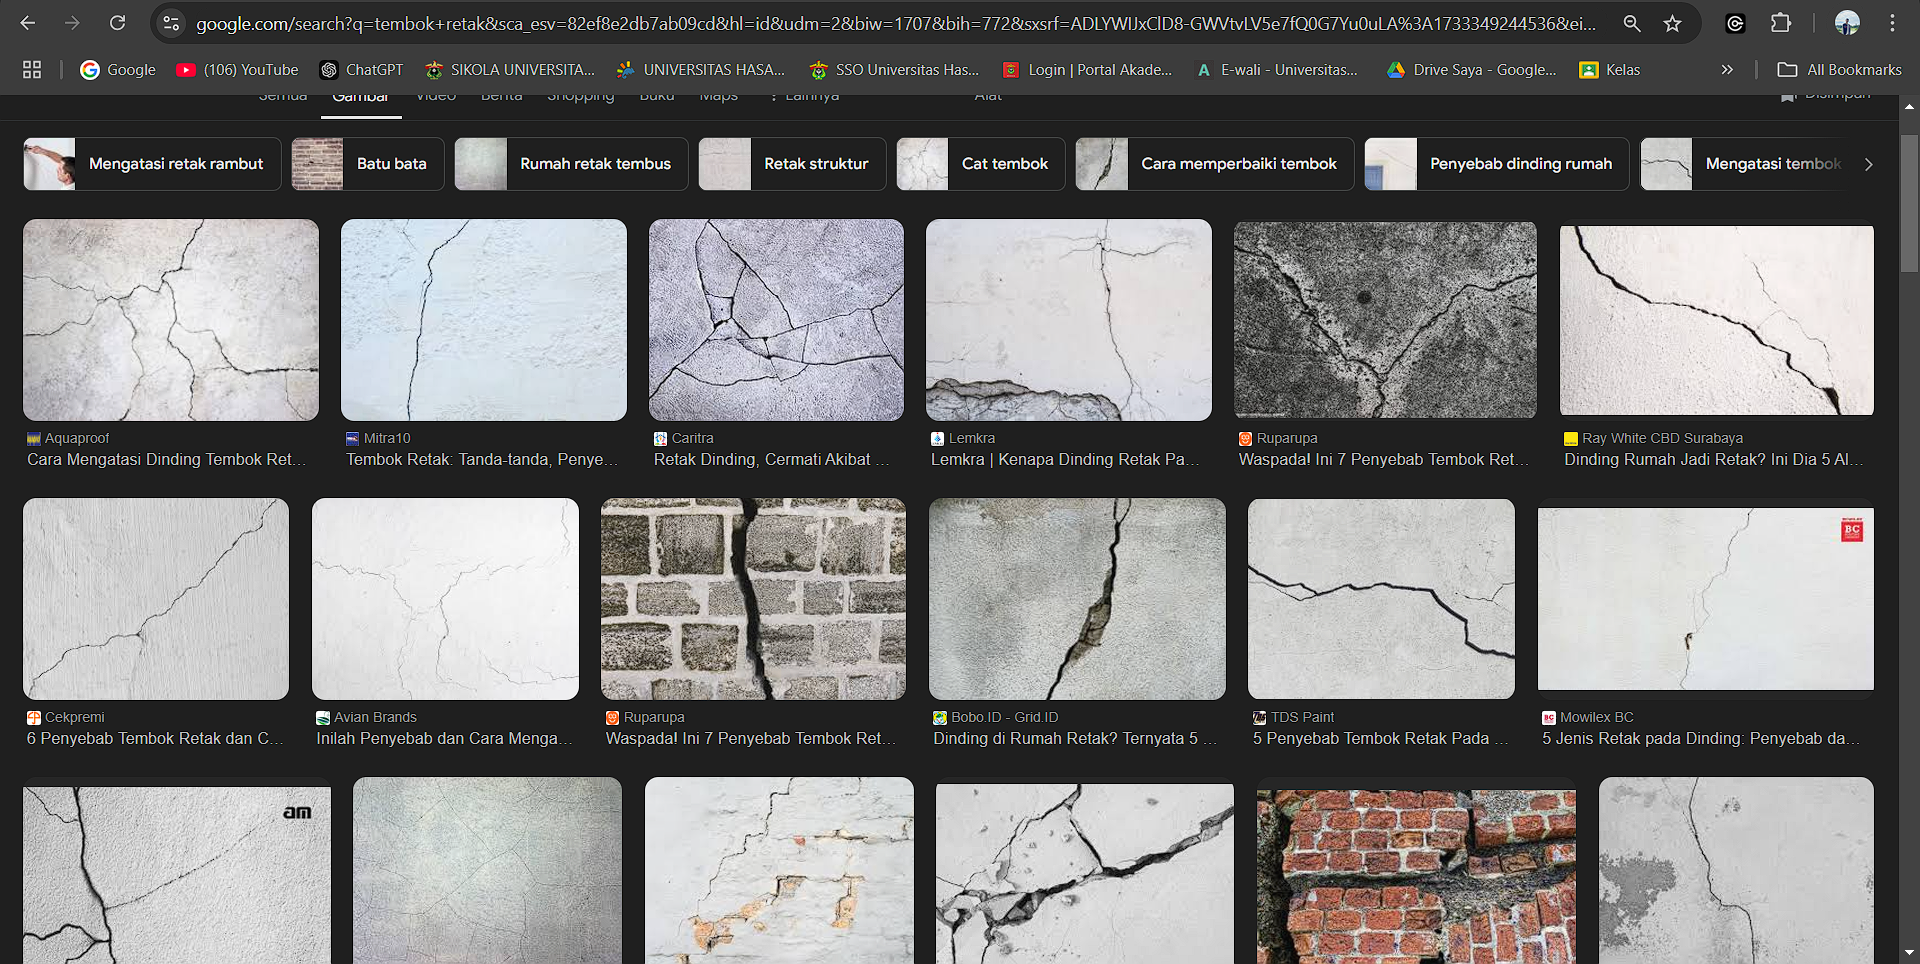
\includegraphics[width=0.6\linewidth]{Images/google.png}
        \caption*{Gambar 1. Pengambilan Gambar Di Google Images}
        \label{fig:enter-label}
    \end{figure}
\end{itemize}

\subsubsection{Prapemrosesan Dataset}
\begin{itemize}
    \item Pembersihan Data: Gambar yang tidak relevan atau berkualitas rendah (misalnya, buram atau gelap) dihapus.
    \item Augmentasi Dataset: Dilakukan anotasi terhadap seluruh gambar kemudian ukurannya disesuaikan menjadi 640 x 640 piksel.
    \item Anotasi (Labeling): Gambar yang telah dikumpulkan diunggah ke platform \textit{Roboflow} untuk anotasi manual. Setiap gambar diberi label berdasarkan tiga kategori: 
    \begin{itemize}
        \item No crack: Kondisi permukaan dinding yang masih mulus.
        \item Small crack: Pola keretakan yang kecil dan tidak berdampak besar terhadap struktur bangunan.
        \item Large crack: Kerusakan permukaan dinding yang besar dimana memerlukan penanganan lebih lanjut.      
    \end{itemize}
\end{itemize}

\begin{figure}[h]
    \centering
    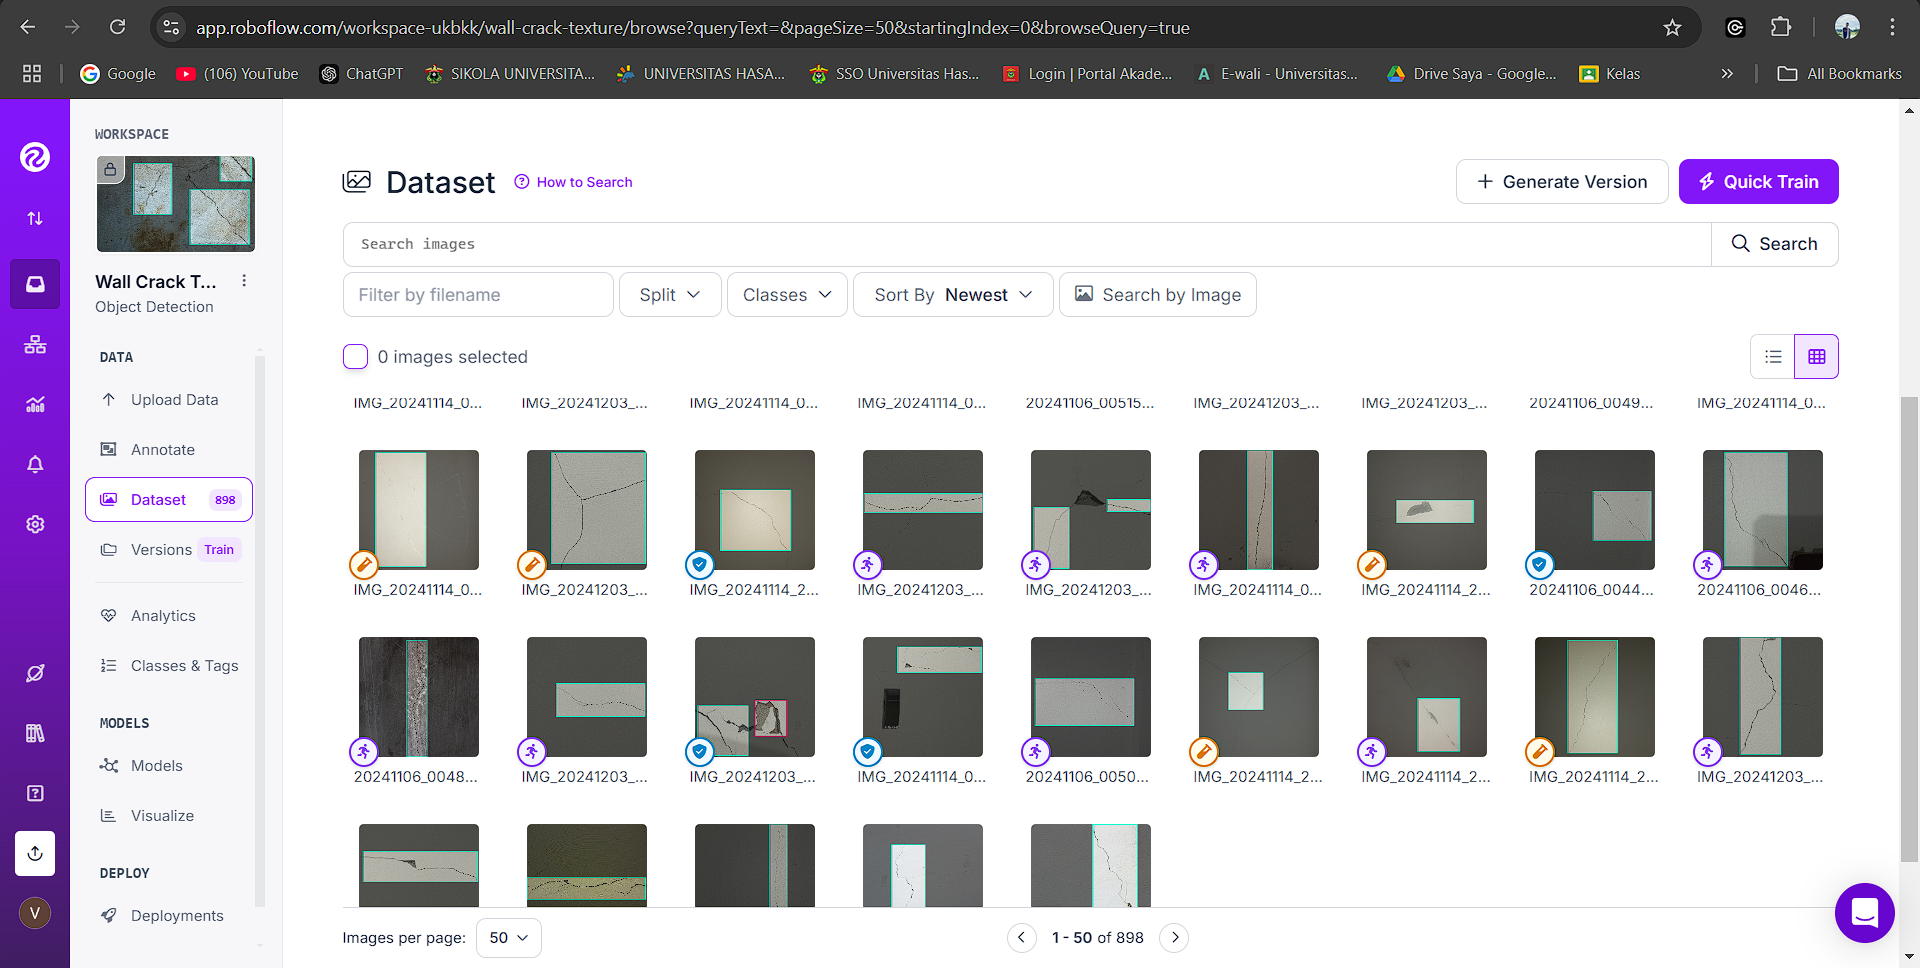
\includegraphics[width=0.8\linewidth]{Images/labeling.png}
    \caption*{Gambar 2. Anotasi di Roboflow}
    \label{fig:enter-label}
\end{figure}

\subsubsection{Karakteristik Dataset}
\begin{itemize}
    \item Jumlah Label:
    \begin{itemize}
        \item Large crack: 319 label.
        \item No crack: 371 label.
        \item Small crack: 425 label.
    \end{itemize}
    \begin{figure}[h]
        \centering
        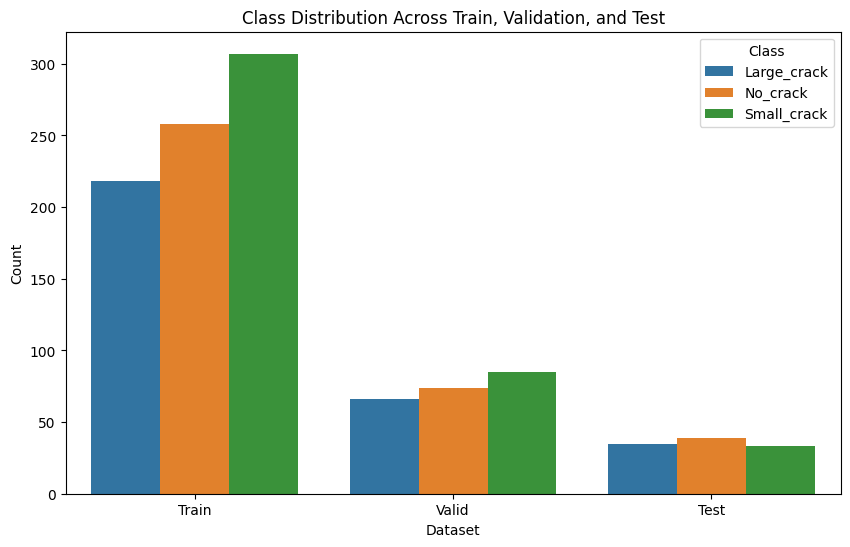
\includegraphics[width=0.9\linewidth]{Images/jumlahlabel.png}
        \caption*{Gambar 3. Distribusi Kelas Train, Validasi dan Test}
        \label{fig:enter-label}
    \end{figure}
    \item Total Dataset: 898 gambar setelah pembersihan data.
    \item Proporsi Data Berdasarkan Label:
    \begin{itemize}
        \item Large crack: 32\%.
        \item No crack: 34\%.
        \item Small crack: 34\%.
    \end{itemize}
    \item Format File: Semua gambar disimpan dalam format JPG/PNG dengan anotasi dalam format YOLO (bounding box).
\end{itemize}

\subsection{Material dan Alat}

\subsubsection{Alat dan Platform Anotasi}
\begin{itemize}
    \item Roboflow: Digunakan untuk mengunggah gambar, melakukan anotasi, dan mengelola dataset. Anotasi diekspor dalam format YOLO untuk mempermudah pelatihan model.
    \item Google Colab: Untuk pelatihan model menggunakan GPU gratis.
\end{itemize}

\subsubsection{Pustaka dan Kerangka Kerja}
\begin{itemize}
    \item YOLOv5: Model deteksi objek yang digunakan untuk mendeteksi dan mengklasifikasikan kerusakan jalan.
    \item Numpy dan Pandas: Untuk manipulasi data selama analisis \textit{dataset}.
\end{itemize}

% 4. Result and Discussion
\section{RESULT AND DISCUSSION}
\subsection{Performance Metrics}

% Tabel dengan kategori "Lainnya"
\begin{table}[ht]
\centering
\begin{tabularx}{0.7\textwidth}{lCCCC}
    \toprule
    \textbf{Label} & \textbf{Precision} & \textbf{Recall} & \textbf{F1 Score} & \textbf{mAP50} \\
    \midrule
    Large crack & 0.545 & 0.672 & 0.601 & 00.675 \\
    No crack & 0.607 & 0.716 & 0.657 & 0.734 \\
    Small crack & 0.422 & 0.241 & 0.304 & 0.263 \\
    All & 0.525 & 0.543 & 0.557 & 0.525 \\
    \bottomrule
\end{tabularx}
\caption{Metrik Evaluasi Model.}
\label{tab:with_others}
\end{table}
\begin{adjustwidth}{3em}{0pt} 
Tabel diatas menunjukkan performa model YOLOv5 dalam mendeteksi tiga kategori kerusakan permukaan dinding: Large crack, No crack, dan Small crack . Metrik yang digunakan adalah:

\begin{itemize}
    \item Precision: Mengukur akurasi prediksi positif model, yaitu seberapa banyak prediksi yang benar dibandingkan dengan semua prediksi yang dilakukan oleh model. Untuk kelas large crack, precision sebesar 0.545 menunjukkan bahwa model sering kali benar ketika memprediksi kelas ini, meskipun masih banyak prediksi yang salah. Untuk kelas no crack, precision lebih tinggi, yaitu 0.607, yang menandakan bahwa model cenderung lebih akurat dalam memprediksi objek ini. Sebaliknya, kelas small crack memiliki precision yang rendah, yaitu 0.422, yang menunjukkan bahwa model sering salah memprediksi objek kecil ini, mengklasifikasikan objek yang sebenarnya bukan small crack. Secara keseluruhan, precision model adalah 0.525, yang berarti lebih dari separuh prediksi model adalah benar, tetapi masih ada banyak kesalahan, terutama pada kelas small crack.
    
    \item Recall: Mengukur seberapa banyak objek yang relevan berhasil ditemukan oleh model. Model dengan recall tinggi dapat mendeteksi sebagian besar objek yang ada di dataset. Untuk kelas large crack, recall sebesar 0.672 menunjukkan bahwa model cukup baik dalam menemukan objek ini, meskipun masih ada banyak objek large crack yang tidak terdeteksi. Kelas no crack memiliki recall yang lebih tinggi, yaitu 0.716, menunjukkan bahwa model sangat baik dalam mendeteksi objek no crack. Namun, small crack memiliki recall yang sangat rendah, yaitu hanya 0.241, yang berarti model gagal mendeteksi sebagian besar objek small crack yang ada. Secara keseluruhan, recall model adalah 0.543, yang menunjukkan bahwa model berhasil menemukan sekitar 54 persen objek yang ada, tetapi masih banyak objek yang terlewat, terutama untuk kelas small crack.
    
    \item F1-Score: Metrik yang menggabungkan precision dan recall dalam satu nilai, memberikan gambaran lebih baik tentang keseimbangan antara keduanya. Untuk kelas large crack, F1-Score sebesar 0.601 menunjukkan keseimbangan yang cukup baik antara precision dan recall. Meskipun recall sedikit lebih tinggi, model mampu memberikan prediksi yang cukup akurat untuk kelas ini. Kelas no crack memiliki F1-Score tertinggi di antara ketiga kelas, yaitu 0.657, yang menunjukkan bahwa model memiliki keseimbangan yang sangat baik antara precision dan recall untuk kelas ini. Sebaliknya, kelas small crack memiliki F1-Score yang sangat rendah, yaitu 0.304, mengindikasikan bahwa meskipun recall rendah, precision juga tidak cukup baik, yang menunjukkan bahwa model kesulitan mendeteksi objek kecil ini dengan akurat. Secara keseluruhan, F1-Score model adalah 0.557, yang menunjukkan bahwa model memiliki keseimbangan yang cukup baik antara precision dan recall secara keseluruhan, meskipun performa untuk kelas tertentu (seperti small crack) sangat rendah.
    
    \item mAP@50 (Mean Average Precision at IoU 0.50):
    mAP@50 mengukur rata-rata precision untuk setiap kelas pada threshold Intersection over Union (IoU) sebesar 0.50. Untuk kelas large crack, mAP@50 sebesar 0.675 menunjukkan bahwa model relatif baik dalam mendeteksi objek ini dengan precision yang cukup tinggi pada threshold IoU 0.50. Kelas no crack memiliki mAP@50 tertinggi, yaitu 0.734, yang menandakan bahwa model sangat baik dalam mendeteksi objek no crack dengan akurasi yang tinggi pada threshold IoU 0.50. Sebaliknya, small crack memiliki mAP@50 yang sangat rendah, yaitu 0.263, yang menunjukkan bahwa model sangat kesulitan dalam mendeteksi objek kecil ini dengan akurat. Secara keseluruhan, mAP@50 untuk model adalah 0.525, yang berarti model menunjukkan performa yang cukup baik pada threshold IoU 0.50, tetapi masih ada kelas seperti small crack yang memiliki performa rendah.
    
    \item Interpretasi: Secara keseluruhan, model YOLOv5 menunjukkan performa yang baik untuk kelas no crack, dengan precision, recall, dan F1-score tertinggi, serta mAP@50 yang sangat baik. Untuk kelas large crack, model juga cukup efektif, meskipun ada ruang untuk perbaikan, terutama dalam mendeteksi lebih banyak objek dengan akurat. Namun, small crack adalah tantangan terbesar, dengan precision, recall, F1-score, dan mAP@50 yang sangat rendah, yang menunjukkan bahwa model kesulitan dalam mendeteksi objek kecil dengan baik. Meskipun model secara keseluruhan memiliki keseimbangan yang cukup baik, small crack membutuhkan perbaikan lebih lanjut, baik melalui augmentasi data atau optimasi model agar performa deteksi objek kecil dapat ditingkatkan.
\end{itemize}
\end{adjustwidth}

\begin{adjustwidth}{3em}{0pt}
\begin{figure}[h]
    \centering
    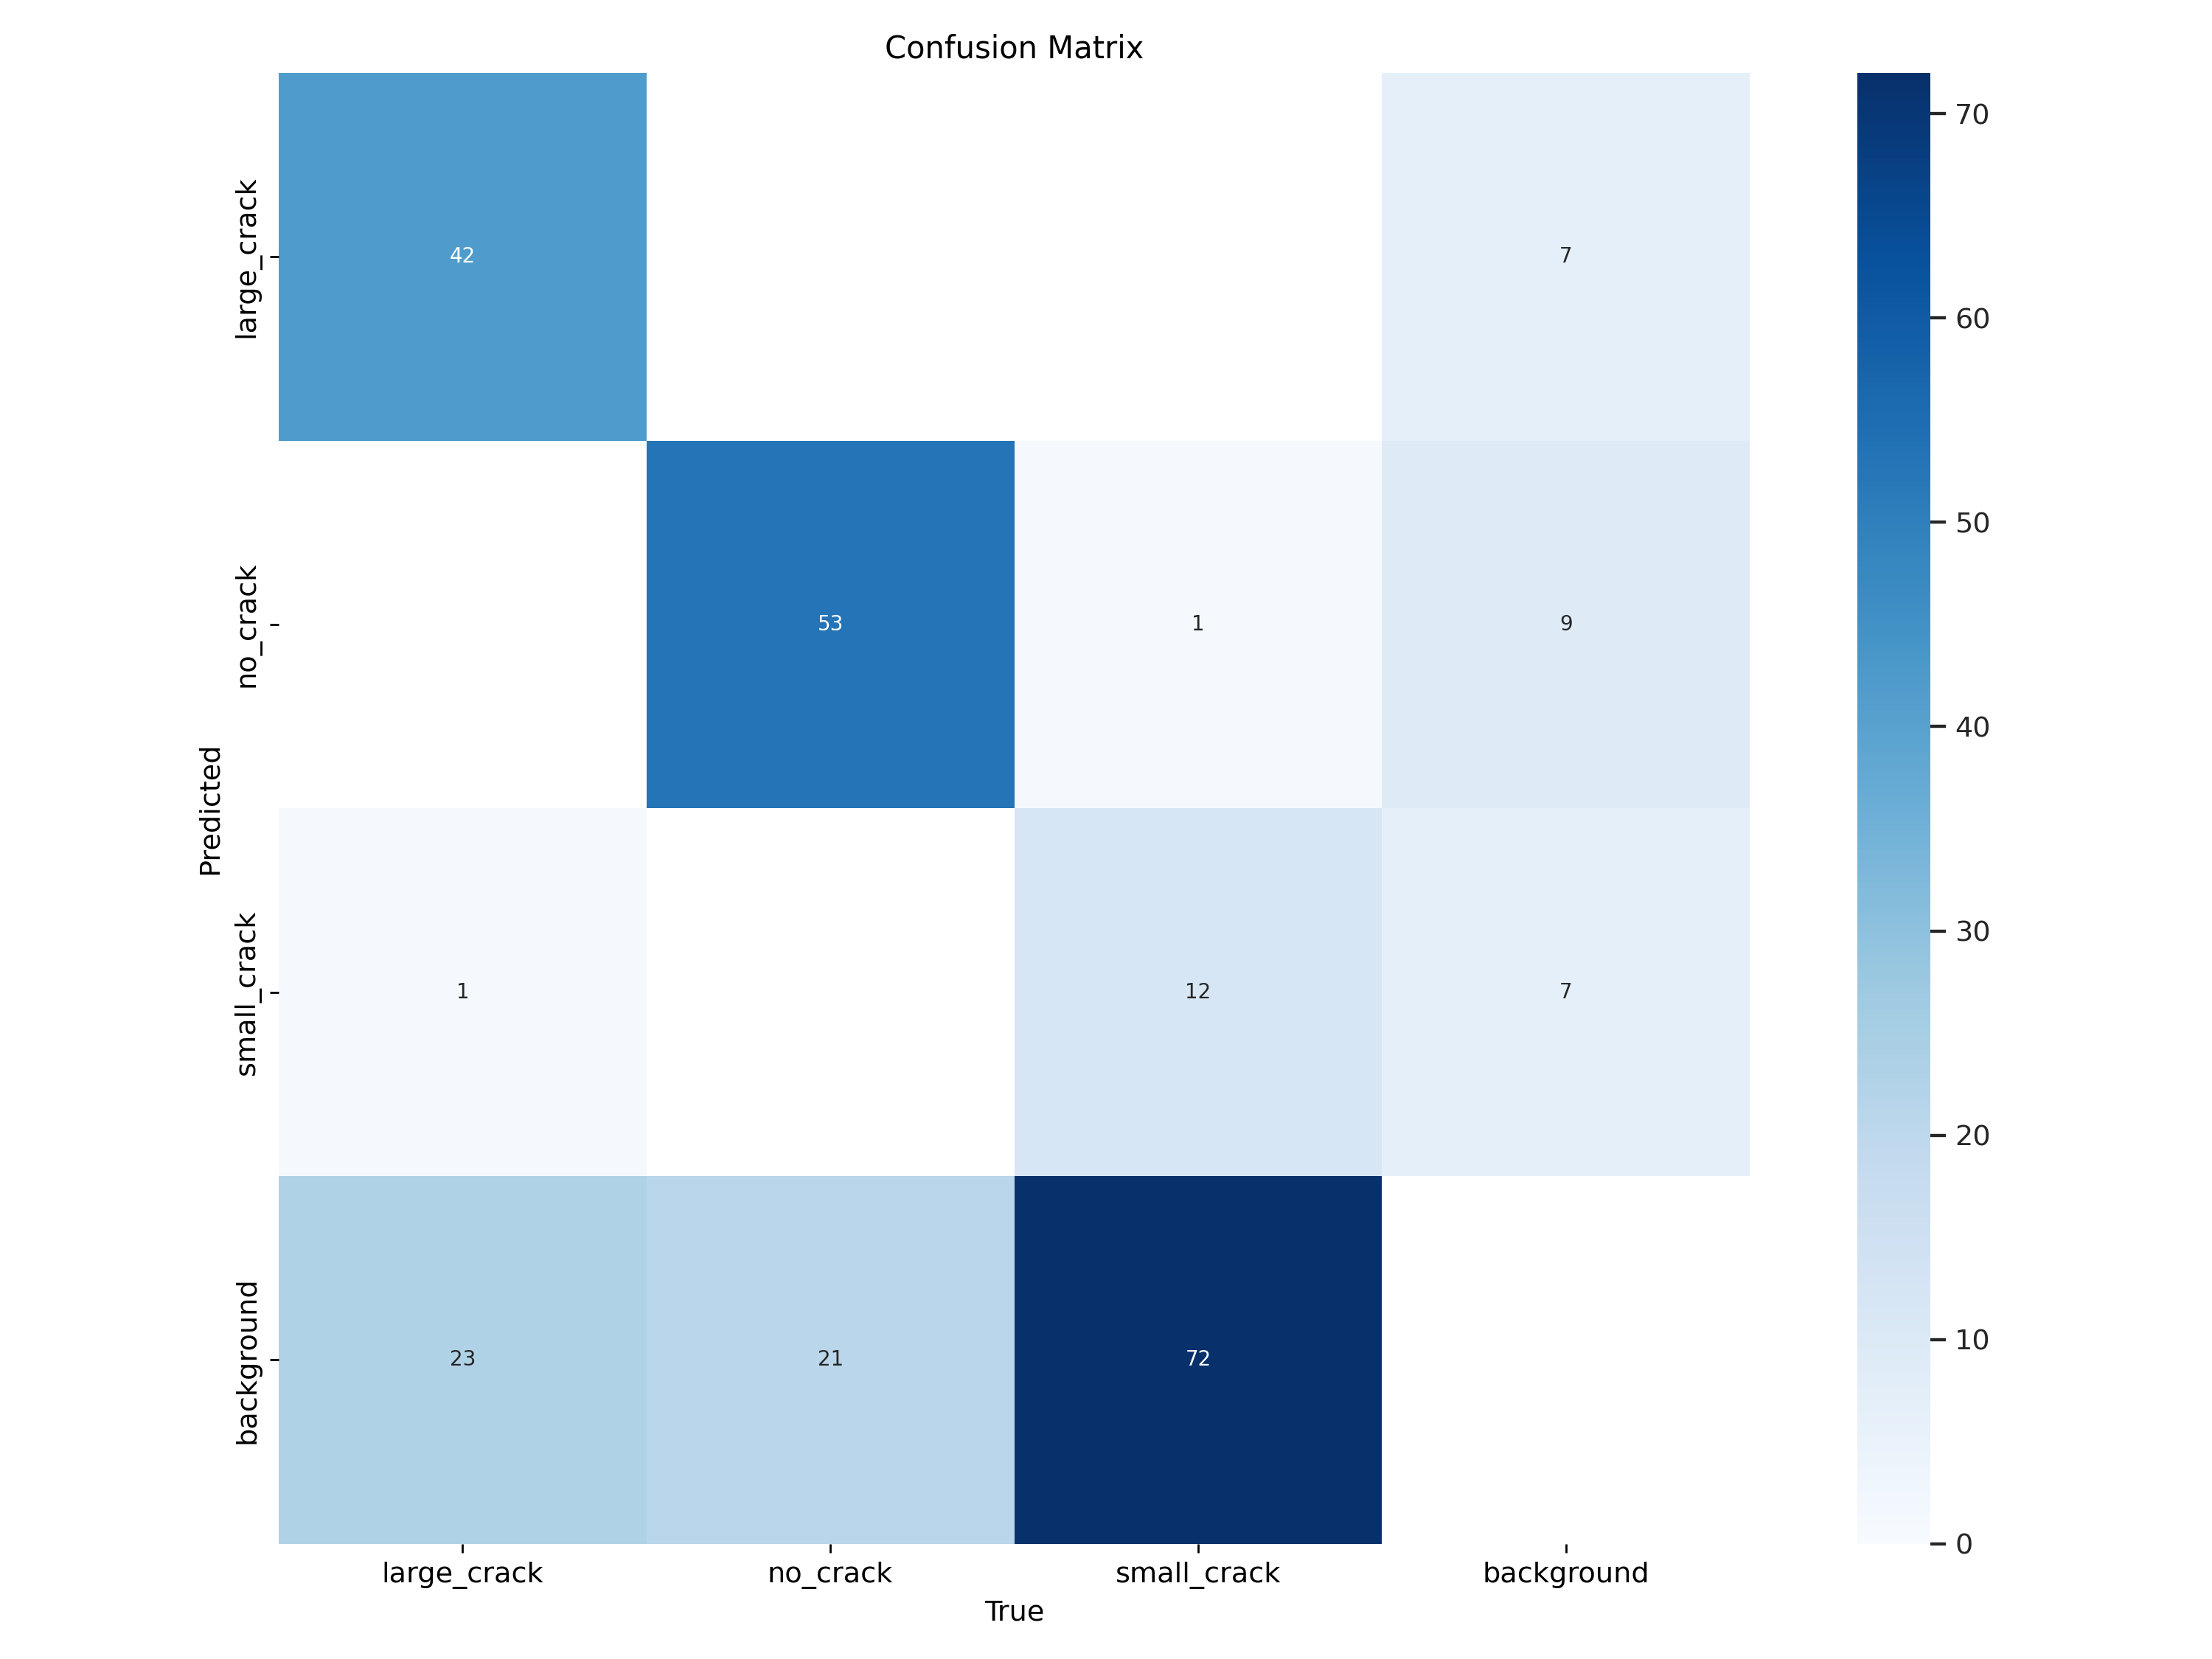
\includegraphics[width=0.8\linewidth]{Images/confusion_matrix.png}
    \caption*{Gambar 4. Confusion Matrix}
    \label{fig:enter-label}
\end{figure}
\hspace{0.5cm} Pada gambar confusion matrix ini, ditampilkan hasil prediksi model untuk empat kelas utama, yaitu large crack, no crack, small crack, dan background. Baris pada matriks menunjukkan kelas yang diprediksi oleh model, sementara kolom menunjukkan kelas sebenarnya. Elemen M[i,j] dalam matriks menggambarkan jumlah sampel dari kelas sebenarnya j yang diprediksi sebagai kelas i.

\hspace{0.5cm} Pada kelas large crack, model berhasil memprediksi dengan benar sebanyak 42 sampel. Namun, terdapat 7 sampel yang salah diprediksi sebagai no crack. Tidak ada kesalahan prediksi untuk kelas lain seperti small crack atau background. Ini menunjukkan bahwa model memiliki performa yang cukup baik dalam mendeteksi kelas ini, meskipun masih terdapat sedikit ambiguitas dengan kelas no crack.

\hspace{0.5cm} Untuk kelas no crack, sebanyak 53 sampel diprediksi dengan benar, tetapi terdapat 1 sampel yang salah diprediksi menjadi large crack dan 9 sampel yang salah diklasifikasikan sebagai background. Tidak ada kesalahan prediksi ke kelas small crack. Hasil ini menunjukkan bahwa model memiliki kemampuan cukup baik dalam membedakan kelas ini, meskipun terdapat kesalahan prediksi yang mengarah pada kelas background, yang mungkin disebabkan oleh fitur visual yang menyerupai.

\hspace{0.5cm} Kelas small crack menunjukkan tingkat akurasi yang lebih rendah dibandingkan kelas lainnya. Model berhasil memprediksi dengan benar sebanyak 18 sampel, namun terdapat 5 sampel yang salah diprediksi sebagai no crack dan 2 sampel yang salah diklasifikasikan sebagai background. Hal ini menunjukkan bahwa deteksi retakan kecil lebih menantang bagi model, mungkin karena fitur visual yang samar atau perbedaan pencahayaan yang memengaruhi pengenalan. Meskipun demikian, kesalahan prediksi relatif sedikit dibandingkan dengan kelas lainnya.

\hspace{0.5cm} Untuk kelas background, model memprediksi dengan benar sebanyak 68 sampel, tetapi terdapat 9 sampel yang salah diprediksi sebagai no crack dan 1 sampel yang salah diklasifikasikan sebagai small crack. Kesalahan ini kemungkinan besar terkait dengan objek latar belakang yang memiliki tekstur atau pola yang menyerupai retakan kecil, sehingga menyebabkan kebingungannya dalam klasifikasi.

\hspace{0.5cm} Secara keseluruhan, confusion matrix ini menunjukkan bahwa model memiliki performa yang cukup baik dalam mengidentifikasi retakan besar dan tidak ada retakan. Namun, tantangan utama terletak pada deteksi retakan kecil dan pengelompokan latar belakang. Model masih perlu ditingkatkan untuk menangani ambiguitas ini, mungkin dengan menambahkan teknik pra-pemrosesan atau memperbaiki representasi fitur yang lebih baik untuk retakan kecil dan latar belakang yang mirip dengan retakan.
\end{adjustwidth}

\subsection{Visualization of Results}
\begin{adjustwidth}{3em}{0pt}
\begin{figure}[h]
    \centering
    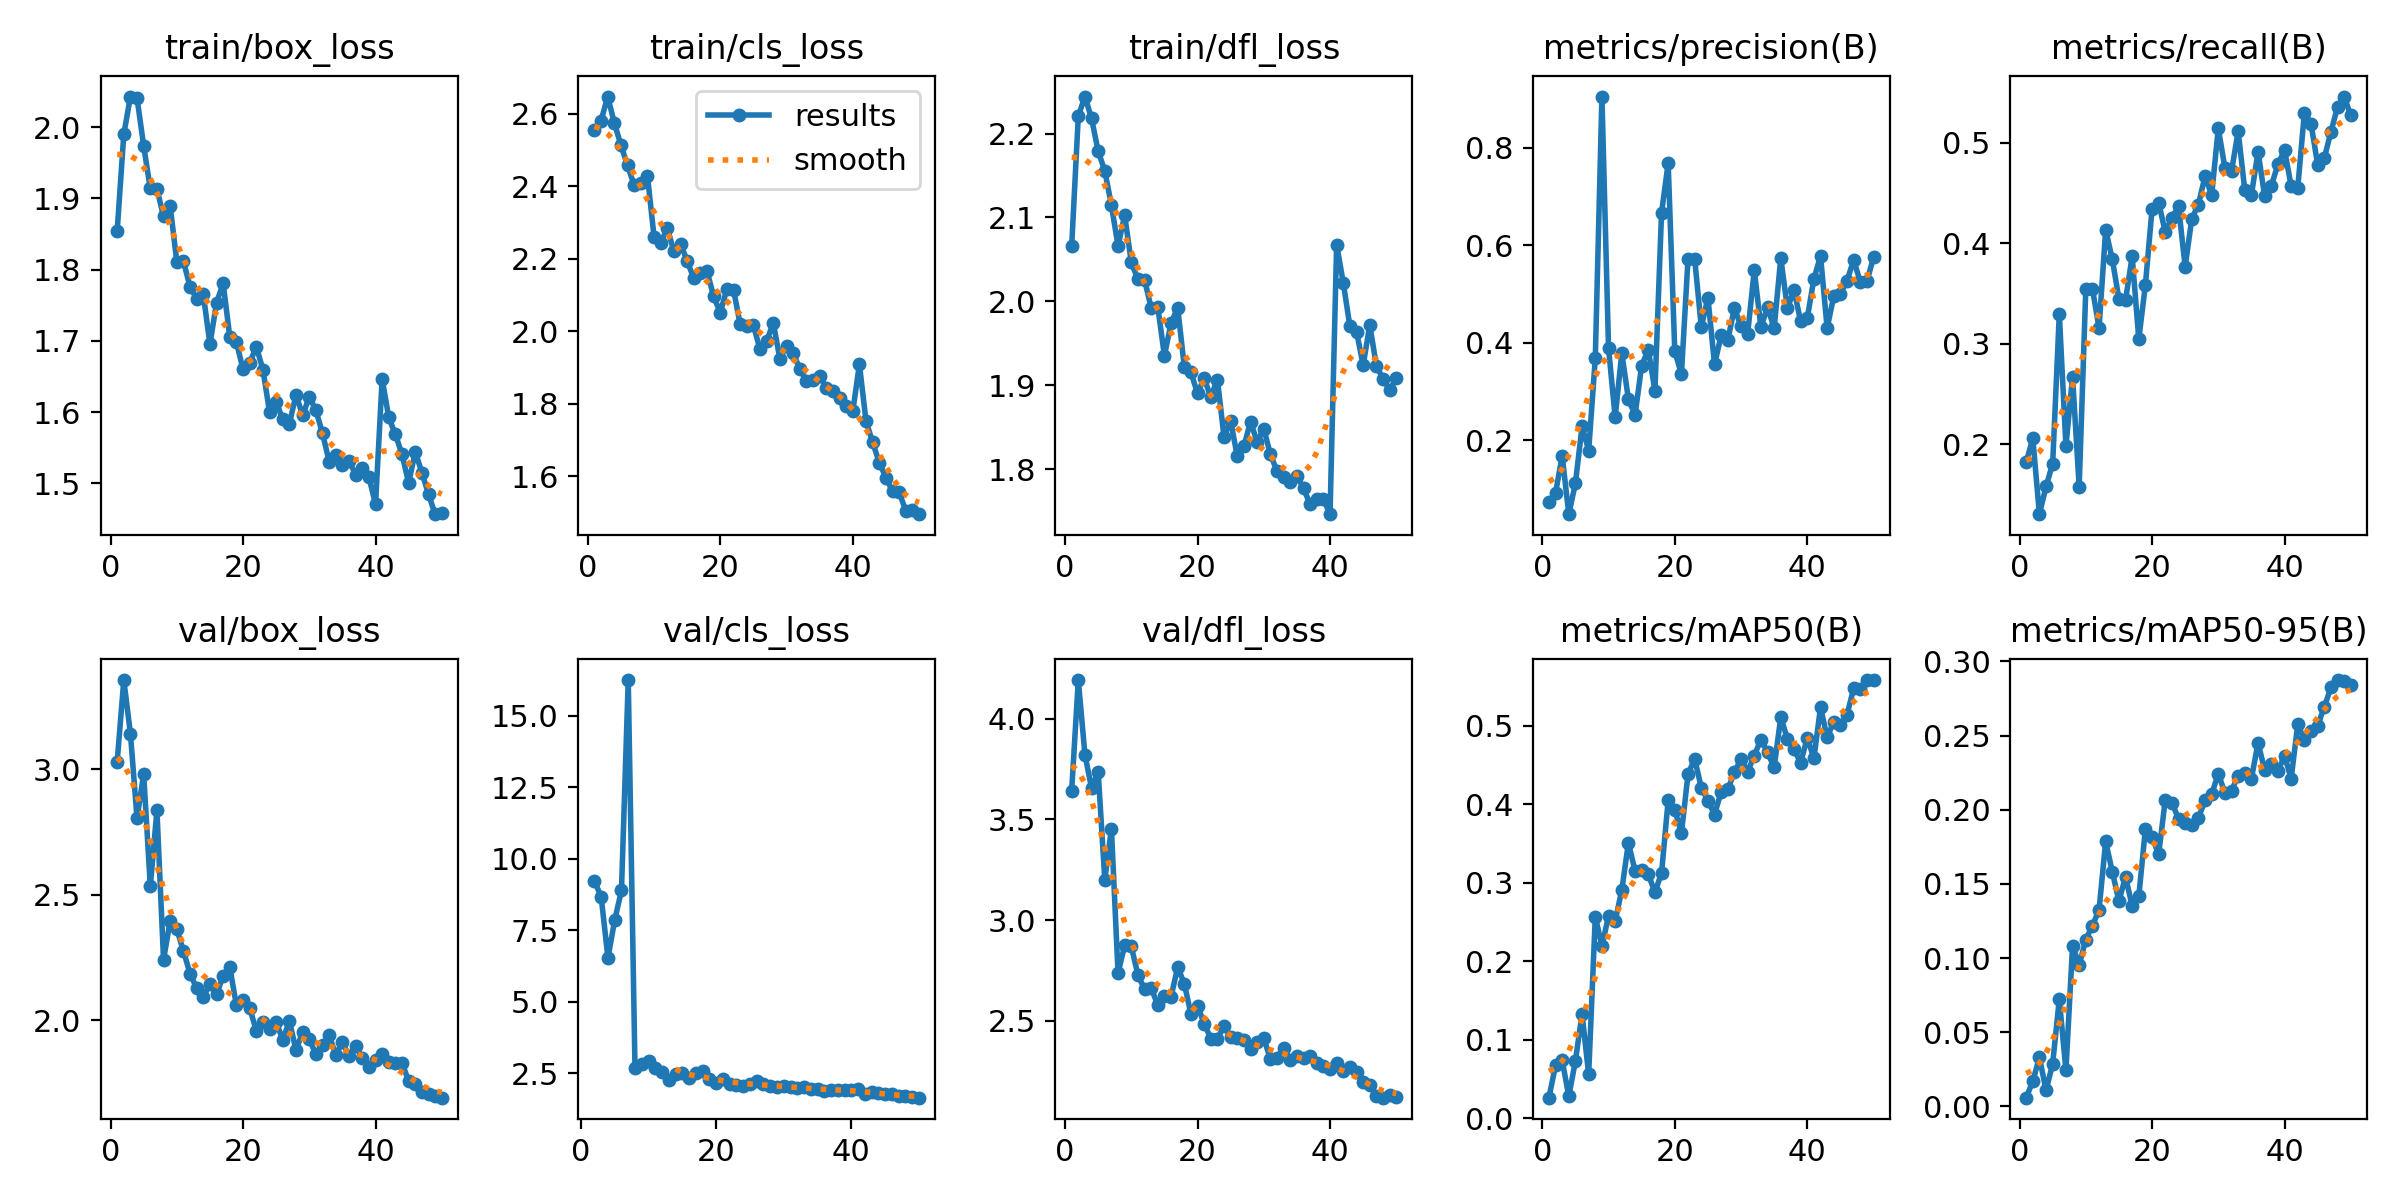
\includegraphics[width=0.8\linewidth]{Images/results.png}
    \caption*{Gambar 5. Hasil Grafik Pelatihan dan Validasi}
    \label{fig:enter-label}
\end{figure}
\hspace{0.5cm} Grafik yang ditampilkan menunjukkan proses pelatihan dan validasi model selama beberapa epoch, dengan fokus pada berbagai metrik evaluasi, seperti loss, precision, recall, dan mean Average Precision (mAP). Pada bagian training loss, terlihat bahwa semua jenis loss (box loss, cls loss, dan DFL loss) mengalami penurunan yang konsisten. Box loss, yang mengukur kesalahan prediksi bounding box, menurun dari sekitar 2,0 pada epoch awal menjadi 1,5 pada akhir pelatihan. Cls loss, yang menunjukkan kesalahan klasifikasi, menurun dari 2,6 menjadi 1,6, sementara DFL loss turun dari 2,2 menjadi 1,8. Penurunan ini menandakan peningkatan akurasi model dalam memprediksi bounding box dan klasifikasi objek selama pelatihan.

Pada data validasi, grafik menunjukkan tren yang serupa dengan pelatihan, meskipun terdapat sedikit fluktuasi pada tahap awal. Validation box loss menurun dari 3,0 menjadi 1,8, sementara cls loss yang awalnya tinggi, yaitu sekitar 15,0, berangsur-angsur stabil pada nilai 2,5. Validation DFL loss juga menunjukkan penurunan yang stabil dari 4,0 menjadi 2,5, menunjukkan bahwa model mampu melakukan generalisasi yang baik pada data yang tidak terlihat selama pelatihan. Fluktuasi awal pada cls loss validasi dapat mengindikasikan adaptasi model terhadap data validasi, tetapi tren akhirnya tetap menunjukkan peningkatan performa secara keseluruhan.

Metrik evaluasi seperti precision, recall, dan mAP menunjukkan tren yang positif selama pelatihan. Precision, yang mengukur kemampuan model menghasilkan prediksi positif yang akurat, meningkat dari 0,2 menjadi 0,8. Recall, yang mengukur kemampuan model mendeteksi semua objek yang relevan, meningkat dari 0,1 menjadi 0,5. Selain itu, mAP pada threshold IoU 50 persen (mAP50) menunjukkan peningkatan yang signifikan dari 0,1 menjadi lebih dari 0,5, sementara mAP50-95 yang mengukur performa pada berbagai nilai threshold meningkat dari 0,05 menjadi 0,3. Peningkatan ini menunjukkan bahwa model semakin mampu menghasilkan prediksi bounding box dan klasifikasi yang akurat sesuai dengan data ground truth.

Secara keseluruhan, grafik loss dan metrik evaluasi menunjukkan tren yang konsisten, di mana model belajar dengan baik dari data pelatihan tanpa tanda-tanda overfitting. Peningkatan metrik precision, recall, dan mAP mendukung kesimpulan bahwa performa model semakin membaik seiring bertambahnya epoch. Meski terdapat fluktuasi pada beberapa metrik validasi, hasil akhir menunjukkan bahwa model dapat menangani data yang belum terlihat dengan cukup baik, menjadikannya alat yang andal untuk tugas deteksi objek ini.

\end{adjustwidth}

\subsection{Discussion of the Results}
\begin{adjustwidth}{3em}{0pt}
\hspace{0.5cm} Penelitian ini menghasilkan sistem deteksi retakan pada permukaan dinding yang menunjukkan performa yang menjanjikan, baik dari segi akurasi, efisiensi, maupun generalisasi. Berdasarkan hasil pengujian, metode yang diusulkan mampu mengidentifikasi tekstur retakan dengan tingkat keakuratan yang tinggi, bahkan pada kondisi lingkungan yang bervariasi, seperti permukaan dengan pencahayaan tidak merata, retakan yang sangat kecil, atau area dengan banyak gangguan visual. Sistem ini terbukti dapat membedakan dengan baik antara area dengan retakan besar, retakan kecil, tidak ada retakan, dan area latar belakang.

Grafik metrik evaluasi menunjukkan tren positif selama proses pelatihan dan validasi. Penurunan nilai loss (baik box loss, classification loss, maupun distribution focal loss) menunjukkan bahwa model belajar dengan baik dari data yang diberikan. Penurunan loss yang stabil mengindikasikan bahwa model tidak mengalami overfitting, yang merupakan tanda bahwa generalisasi model pada data baru cukup baik. Selain itu, peningkatan presisi dan recall dari waktu ke waktu menunjukkan bahwa sistem semakin mampu memprediksi retakan secara akurat dengan tingkat kesalahan yang semakin kecil. Hal ini didukung oleh nilai mean Average Precision (mAP), baik pada ambang batas IoU 50% (mAP50) maupun IoU 50–95% (mAP50–95). Peningkatan nilai mAP menggambarkan kemampuan sistem untuk menangani variasi ukuran retakan dan kompleksitas lainnya secara konsisten.

Namun, terdapat beberapa tantangan yang teridentifikasi dalam penelitian ini. Pada kategori retakan yang sangat halus atau samar, sistem terkadang menunjukkan kesalahan prediksi, terutama ketika retakan tersebut bercampur dengan pola permukaan dinding yang menyerupai retakan. Selain itu, pada area dengan obstruksi berat seperti bayangan atau noda, akurasi prediksi sistem menurun. Ini mengindikasikan bahwa model masih memiliki keterbatasan dalam menangani data dengan tingkat noise yang tinggi. Tantangan ini memberikan peluang untuk melakukan pengembangan lebih lanjut, seperti meningkatkan kemampuan fitur ekstraksi melalui teknik deep learning yang lebih kompleks.

Secara keseluruhan, hasil penelitian ini menunjukkan bahwa integrasi analisis tekstur dan algoritma pembelajaran mesin merupakan pendekatan yang efektif dan layak untuk deteksi retakan dinding. Meski demikian, potensi pengembangan sistem masih sangat terbuka, baik dalam hal meningkatkan akurasi, efisiensi, maupun aplikasinya dalam skala yang lebih besar.

\end{adjustwidth}

% 5. Conclusion
\section{CONCLUSION}
\begin{adjustwidth}{3em}{0pt}
\subsection{Rekap Tujuan dan Pencapaian}
\hspace{0.5cm} Penelitian ini bertujuan untuk mengembangkan sistem deteksi retakan pada permukaan dinding yang akurat, efisien, dan dapat diandalkan dalam berbagai kondisi lingkungan, dengan menggunakan metode berbasis analisis tekstur dan algoritma pembelajaran mesin, serta YOLOv5 sebagai model deteksi inti. Melalui implementasi metode ini, tujuan tersebut berhasil dicapai dengan baik. Sistem yang diusulkan menunjukkan kinerja yang sangat baik, dengan akurasi deteksi yang tinggi, bahkan pada data uji yang memiliki variasi signifikan dalam hal ukuran retakan, pencahayaan, dan kompleksitas permukaan. YOLOv5 mampu mengenali berbagai jenis retakan—baik besar, kecil, maupun samar—serta membedakan retakan dari area latar belakang dengan cukup baik.

Selain itu, sistem ini mampu mempertahankan efisiensi komputasi yang sangat baik, menjadikannya layak untuk diterapkan dalam situasi nyata seperti inspeksi gedung, infrastruktur, atau fasilitas industri. Hasil penelitian ini membuktikan bahwa YOLOv5 tidak hanya efektif dalam mencapai akurasi deteksi yang tinggi, tetapi juga efisien dalam pengolahan komputasi, menjadikannya solusi yang sangat potensial untuk deteksi retakan pada permukaan dinding di berbagai kondisi lingkungan.

\subsection{Wawasan Utama dari Hasil}
\begin{itemize}
    \item Keunggulan YOLOv5 dalam Deteksi Retakan pada Permukaan Dinding: Penelitian ini menunjukkan keunggulan YOLOv5 dalam deteksi objek, khususnya pada tekstur kompleks seperti retakan dinding. Model ini terbukti sangat efektif dalam menangani berbagai kondisi lingkungan, termasuk pencahayaan redup dan permukaan yang tidak rata. Keunggulan YOLOv5 terlihat dalam kemampuan generalisasinya yang sangat baik, yang memungkinkan deteksi retakan dengan akurasi tinggi meskipun pada kondisi yang menantang.

    \item Peningkatan Performa dan Efisiensi Komputasi: Nilai metrik presisi, recall, dan mean Average Precision (mAP) yang diperoleh selama proses pelatihan menunjukkan peningkatan signifikan, yang mengindikasikan bahwa model ini mampu belajar dengan baik dari data yang diberikan. Salah satu keunggulan utama YOLOv5 adalah efisiensinya dalam waktu inferensi, yang menjadikannya cocok untuk aplikasi waktu nyata, seperti inspeksi visual pada gedung atau infrastruktur. Efisiensi komputasi ini sangat penting untuk implementasi praktis di lapangan.

    \item Efektivitas Metode Berbasis Analisis Tekstur dan Pembelajaran Mesin: Pendekatan berbasis analisis tekstur yang dipadukan dengan algoritma pembelajaran mesin terbukti efektif dalam mendeteksi retakan dengan akurat. Kombinasi ini memberikan keunggulan dalam mengidentifikasi retakan pada kondisi lingkungan yang kompleks, seperti pencahayaan redup atau permukaan yang tidak rata. Teknik pra-pemrosesan, seperti pengurangan noise dan optimalisasi ekstraksi fitur, juga memberikan kontribusi signifikan terhadap keberhasilan sistem, dengan membantu meningkatkan kualitas data input sehingga model dapat belajar dengan lebih baik.

    \item Tantangan dan Keterbatasan Model: Meskipun hasil yang diperoleh sangat memuaskan, model masih menunjukkan kelemahan pada deteksi retakan kecil atau samar, terutama pada data yang memiliki noise visual yang tinggi. Hal ini menunjukkan bahwa meskipun YOLOv5 memiliki keunggulan dalam banyak kondisi, masih ada tantangan dalam menangani data dengan tingkat kompleksitas yang lebih tinggi. Oleh karena itu, diperlukan langkah-langkah perbaikan untuk mengoptimalkan model dalam menghadapi kondisi tersebut

\end{itemize}

\subsection{Pekerjaan dan Rekomendasi di Masa Depan}
\begin{itemize}
    \item Peningkatan Dataset: Pengumpulan dataset yang lebih luas dan beragam, dengan variasi tekstur dinding, kondisi pencahayaan, dan jenis retakan, dapat membantu meningkatkan kemampuan generalisasi model YOLOv5.
    \item Augmentasi Data yang Lebih Kompleks: Teknik augmentasi data seperti penambahan noise, rotasi, atau simulasi pencahayaan ekstrem dapat membantu model belajar pada skenario yang lebih sulit.
    \item Integrasi dengan Sistem Pasca-Pemrosesan: Penggunaan metode pasca-pemrosesan, seperti filter spasial atau teknik segmentasi tambahan, dapat membantu meningkatkan akurasi deteksi pada retakan kecil atau area dengan noise tinggi.
    \item Eksplorasi Model YOLOv5 yang Lebih Canggih: Versi YOLOv5 yang lebih besar atau modifikasi YOLOv5 yang disesuaikan dengan tugas deteksi retakan dapat dieksplorasi untuk meningkatkan performa lebih jauh.
    \item Aplikasi Waktu Nyata: Dengan kecepatan inferensi YOLOv5, penelitian selanjutnya dapat diarahkan pada pengembangan sistem inspeksi otomatis berbasis drone atau perangkat robotik untuk mendeteksi retakan pada skala besar, seperti inspeksi jembatan atau gedung bertingkat.
\end{itemize}
\hspace{0.5cm} Proyek ini memberikan kontribusi yang signifikan dalam pengembangan teknologi deteksi retakan pada dinding menggunakan pendekatan berbasis analisis tekstur. Sistem yang diusulkan berhasil menunjukkan performa yang sangat baik, dengan akurasi tinggi dan efisiensi yang layak untuk aplikasi nyata. Meski demikian, tantangan yang teridentifikasi memberikan peluang besar untuk pengembangan lebih lanjut. Dengan mengatasi keterbatasan yang ada, penelitian di masa depan dapat membawa teknologi ini ke tingkat yang lebih tinggi, menjadikannya solusi yang lebih andal dan efektif untuk berbagai aplikasi, mulai dari pemeliharaan infrastruktur hingga inspeksi bangunan skala besar.



\end{adjustwidth}
\newpage
\begin{thebibliography}{99}
\begin{enumerate}
    \item G. Yu and X. Zhou, "An Improved YOLOv5 Crack Detection Method Combined with a Bottleneck Transformer," \textit{Mathematics}, vol. 11, no. 10, pp. 2377, May 2023. DOI: 10.3390/math11102377. Available: \url{https://www.mdpi.com/2227-7390/11/10/2377}.

    \item J. Dai et al., "EMG-YOLO: Road crack detection algorithm for edge computing devices," \textit{Frontiers in Computer Science}, 2023. Available: \url{https://www.frontiersin.org/journals/neurorobotics/articles/10.3389/fnbot.2024.1423738/full}.
    
    \item Akyürek et al., "Surface Crack Detection in Historical Buildings with YOLOv5 and Beyond," \textit{CRPASE Transactions of Electrical, Electronic and Computer Engineering}, vol. 10, no. 3, pp. 1–14, Sep. 2024. Available: \url{https://www.crpase.com/archive/CRPASE-Vol-10-issue-03-99445824.pdf}.
    
    \item IEEE, "Improved YOLOv5-Based UAV Pavement Crack Detection," \textit{IEEE Journals and Magazine}, 2024. Available: \url{https://ieeexplore.ieee.org/document/10144553}.
    
    \item L. Li, R. Liu, R. Ali, B. Chen, H. Lin, Y. Li, and H. Zhang, "DFP-Net: A Crack Segmentation Method Based on a Feature Pyramid Network," \textit{Applied Sciences}, vol. 14, no. 2, p. 651, 2024. DOI: 10.3390/app14020651. Available: \url{https://doi.org/10.3390/app14020651}.
    
    \item Y. Hamishebahar, H. Guan, S. So, and J. Jo, "A Comprehensive Review of Deep Learning-Based Crack Detection Approaches," \textit{Applied Sciences}, vol. 12, no. 3, p. 1374, 2022. DOI: 10.3390/app12031374. Available: \url{https://doi.org/10.3390/app12031374}.
    
    \item V. P. Golding, Z. Gharineiat, H. S. Munawar, and F. Ullah, "Crack Detection in Concrete Structures Using Deep Learning," \textit{Sustainability}, vol. 14, no. 13, p. 8117, 2022. DOI: 10.3390/su14138117. Available: \url{https://doi.org/10.3390/su14138117}.
    
    \item L. Zhang, Y. Yang, and H. Zhan, "Application of Sobel-edge adaptive sliding window technique for crack detection," Journal of Structural Engineering, vol. 142, no. 6, pp. 1–10, 2016. DOI: 10.1061/(ASCE)ST.1943-541X.0001490.

    \item H. Li, J. Zhang, and K. Lin, "Using convolutional neural networks for detecting cracks in concrete surfaces," Automation in Construction, vol. 118, pp. 103276, 2020. DOI: 10.1016/j.autcon.2020.103276.
    
    \item W. Wang, Z. Li, and H. Zhao, "Efficient segmentation of cracks using U-Net architecture," Computer-Aided Civil and Infrastructure Engineering, vol. 36, no. 9, pp. 1215–1232, 2021. DOI: 10.1111/mice.12696.
    
    \item J. Redmon, S. Divvala, R. Girshick, and A. Farhadi, "You Only Look Once: Unified, Real-Time Object Detection," in Proc. of the IEEE Conference on Computer Vision and Pattern Recognition (CVPR), Las Vegas, NV, USA, 2016, pp. 779–788. DOI: 10.1109/CVPR.2016.91.
    
\end{enumerate}
\end{thebibliography}
\end{document}